%%\documentclass[pdflatex,sn-basic,Numbered]{sn-jnl}% Basic, numbered refs
%%\documentclass[twocolumn,pdflatex,sn-basic]{sn-jnl}% Basic, two column unnumbered refs
\documentclass[pdflatex,sn-basic]{sn-jnl}% Basic, one column unnumbered refs
%%\documentclass[referee,sn-basic]{sn-jnl}% referee option is meant for double line spacing

%%%% Standard Packages
%%<additional latex packages if required can be included here>

\usepackage{graphicx}%
\usepackage{multirow}%
\usepackage{amsmath,amssymb,amsfonts}%
\usepackage{amsthm}%
\usepackage{mathrsfs}%
\usepackage[title]{appendix}%
\usepackage{xcolor}%
\usepackage{textcomp}%
\usepackage{manyfoot}%
\usepackage{booktabs}%
\usepackage{algorithm}%
\usepackage{algorithmicx}%
\usepackage{algpseudocode}%
\usepackage{listings}%
% \usepackage{lmodern}%
\usepackage{anyfontsize}%
\usepackage{siunitx}%
%%%%

\raggedbottom
\unnumbered% uncomment this for unnumbered level heads

% Zach's commands

% Units
\DeclareSIUnit\molar{\textsc{m}}
\DeclareSIUnit\uM{\micro\molar}
\DeclareSIUnit\nM{\nano\molar}
\DeclareSIUnit\angstrom{\text {Å}}

% Taxonomy
\newcommand\ec{\textit{E.~coli}}
\newcommand\ecfull{\textit{Escherichia coli}}
% \newcommand\mtb{\textit{M.~tuberculosis}}
\newcommand\mtb{Mtb}
\newcommand\mtbfull{\textit{Mycobacterium tuberculosis}}
\newcommand\msmegfull{\textit{Mycolicibacterium smegmatis}}
\newcommand\pafull{\textit{Pseudomonas aeruginosa}}

% Protein variant and region designations
\newcommand\ftsbTM{FtsB\textsuperscript{TM}}
\newcommand\ftsbLQ{FtsB\textsuperscript{LQ}}
\newcommand\ftsbH{FtsB\textsuperscript{H}}
\newcommand\ftsbdLQ{FtsB\textsuperscript{$\Delta{}$LQ}}
\newcommand\ftsbdH{FtsB\textsuperscript{$\Delta{}$H}}
\newcommand\ftsbdLQdH{FtsB\textsuperscript{$\Delta{}$LQ$\Delta{}$H}}
\newcommand\permN{PerM\textsuperscript{n1}}

\begin{document}

% Temp to fill in dummy text
\newcommand\loremipsum{\textcolor{lightgray}{Lorem ipsum dolor sit amet, consectetur adipiscing elit. Nulla volutpat lacus vitae arcu blandit, in maximus arcu bibendum. Aliquam posuere enim et sem egestas gravida. In hac habitasse platea dictumst. Praesent non risus justo. Nullam rhoncus elit in fermentum ultrices. Quisque luctus suscipit lectus in lacinia. Mauris mauris mauris, pretium vitae malesuada id, fringilla aliquet ex. In hac habitasse platea dictumst. Vivamus scelerisque, nulla in euismod placerat, dolor purus commodo tortor, quis congue risus purus nec tellus. Phasellus ultricies lacinia tristique. Duis sollicitudin sapien a nisi sagittis sodales. Suspendisse consequat mauris quis ante consequat tincidunt. Vivamus volutpat in mi vel dictum. Ut ac ligula lectus. Duis ullamcorper ex vitae imperdiet pellentesque. Vestibulum id massa interdum, posuere nibh non, consequat leo.}}

\title[Article Title]{\mtbfull{} FtsB and PerM interact via a C-terminal helix in FtsB to modulate cell division}

\author[1]{\fnm{João Ramalheira} \sur{Ferreira}}
\equalcont{These authors contributed equally to this work.}

\author[1]{\fnm{Ruilan} \sur{Xu}}
\equalcont{These authors contributed equally to this work.}

\author*[1]{\fnm{Zach} \sur{Hensel}}\email{zach.hensel@itqb.unl.pt}

\affil[1]{\orgdiv{ITQB NOVA}, \orgname{Universidade NOVA de Lisboa}, \orgaddress{\street{Av. da República}, \city{Oeiras}, \postcode{2780-157}, \country{Portugal}}}

\abstract{Latent infection by \mtbfull{} (\mtb{}) impedes effective tuberculosis therapy and eradication. The protein PerM is essential for chronic \mtb{} infections in mice and acts via the divisome protein FtsB to modulate cell division. Using transgenic co-expression in \ecfull{}, we studied the \mtb{} PerM-FtsB interaction in isolation from other \mtb{} proteins, engineering PerM to enhance expression in the \ec{} membrane. We confirmed the reported instability of \mtb{} FtsB, and we linked FtsB instability to a segment of FtsB predicted to bind cell-division proteins FtsL and FtsQ. Though narrowly conserved, the PerM-FtsB interaction emerges as a potential target as part of therapy targeting persistent infections by disrupting regulation of cell division. Using fluorescence microscopy, we found that the stability of both FtsB and PerM hinges on their interaction via a C-terminal helix in FtsB. Molecular dynamics results supported the observation that FtsB stabilized PerM, and suggested that interactions at the PerM-FtsB interface differ from our initial structure prediction in a way that is consistent with PerM sequence conservation. Integrating protein structure prediction, molecular dynamics and single-molecule microscopy, our approach is primed to screen potential inhibitors of the PerM-FtsB interaction and can be straightforwardly adapted to explore other putative interactions.}

\keywords{\mtbfull{}, cell division, single-molecule microscopy, molecular dynamics}

\maketitle

\section{Introduction}\label{sec1}

\mtbfull{} (\mtb{}) is a major contributor to preventable deaths by infectious disease and has infected approximately a quarter of the global population \citep{houbenGlobalBurdenLatent2016}. Most infections progress to latent tuberculosis infection (LTBI), characterized by an immunological response to \mtb{} antigens without clinical signs of active TB \citep{whoLatentTuberculosisInfection2018}. Preventing establishment and reactivation of LTBI is a growing priority for TB elimination strategies, although uncertainties continue to limit measurements of the relative burdens of new TB infections and LTBI reactivation \citep{daleQuantifyingRatesLate2021}. Protocols that reduce the duration and adverse effects of treatment can reduce LTBI burden by improving upon completion rates for preventative treatment \citep{assefaEfficacySafetyDifferent2023}. Furthermore, imperfect treatment over long periods can contribute to acquisition of drug resistance \citep{liAcquiredResistanceIsoniazid2021}. Consequently, it is imperative to better understand how \mtb{} infections persist to establish LTBI to inform strategies for novel LTBI treatments with higher efficacy, shorter durations, and reduced risk of drug resistance.

A potential strategy to prevent establishment and reactivation of LTBI is to characterize and target mechanisms through which \mtb{} persists through host-induced stress \citep{dartoisAntituberculosisTreatmentStrategies2022}. The actinomycete protein PerM was one of 21 genes identified in a screen of transposon \mtb{} mutants with attenuated growth at pH~$4.5$ in media containing Tween 80, with most of the identified genes being associated with cell wall synthesis \citep{vandalMembraneProteinPreserves2008}. A subsequent study focused on PerM, finding that \mtb{} PerM knockout reduced growth during chronic mouse infection and increased $\beta$-lactam antibiotic susceptibility. Localization of fluorescently tagged PerM to dividing septa suggested a connection to cell division \citep{goodsmithDisruptionTuberculosisMembrane2015}. Further work demonstrated that PerM associates with the \mtb{} divisome, a protein complex orchestrating cell wall remodeling during division, and that PerM depletion can be complemented by overexpression of the divisome component FtsB \citep{wangPersistentMycobacteriumTuberculosis2019}. PerM was also recently identified by transposon sequencing to play an even more significant role in infecting mice in a background with weakened adaptive immune response \citep{meadeGenomewideScreenIdentifies2023}.

Recently, a covalent inhibitor of divisome formation based upon the structure of FtsB-FtsQ was developed and found to be active against drug-resistant \ec{} in an animal infection model \citep{paulussenCovalentProteomimeticInhibitor2022}. The \mtb{} proteome includes homologs of the five core \ec{} divisome proteins FtsQ, FtsL, FtsB, FtsW, and FtsI \citep{wuCharacterizationConservedNovel2018}, suggesting that a similar approach can target protein-protein interactions in the \mtb{} divisome. However, it is unknown whether PerM directly interacts with FtsB  \citep{wangPersistentMycobacteriumTuberculosis2019} and, if it does, whether there is a regulatory mechanism for PerM beyond impacting FtsB stability. PerM lacks known orthologs outside of actinomycetes \citep{goodsmithDisruptionTuberculosisMembrane2015}, so PerM interactions could potentially be targets of specific therapy. However, no experimental structural data have been published on the PerM-FtsB interaction or on PerM alone to guide experimental design. Expression and purification of \mtb{} PerM and FtsB for structural study is likely to pose difficulties given that FtsB stability depends upon PerM co-expression in \mtb{} and \msmegfull{} \citep{wangPersistentMycobacteriumTuberculosis2019}. Furthermore, proteins such as PerM with a high number of transmembrane helices pose challenges for recombinant expression \citep{graveHighthroughputStrategyIdentification2022, korepanovaCloningExpressionMultiple2005}.

Recent insights into the molecular structure and regulatory mechanisms of the gram-negative divisome have been enabled by the confluence of protein structure prediction, cryogenic electron microscopy (Cryo-EM), and molecular dynamics (MD) simulations. The extension from prediction of monomers to protein complexes \citep{baekAccuratePredictionProtein2021, evansProteinComplexPrediction2022} facilitated rapid structure prediction of the core \ec{} divisome \citep{attaibiUpdatedModelDivisome2022, cravenModelInteractionsFtsQLB2022}. Analysis of a Cryo-EM structure of the \pafull{} divisome was largely consistent with predicted protein-protein interfaces, but also revealed a global conformational change absent in structure predictions \citep{kashammerCryoEMStructureBacterial2023}. All-atom MD simulations identified this conformational change within 1 $\mu$s, and further predicted interactions between the core divisome and \ec{} FtsN \citep{brittonConformationalChangesEssential2023}. However, limitations of this MD approach, such as uncertainty in structure predictions and limited MD timescales, call for experimental validation. Importantly, in silico predictions for FtsN were corroborated by experimental results in living cells \citep{parkEssentialDomainFtsN2023}.

In this work, we employed a combination of structure prediction, MD, and fluorescence microscopy to probe the predicted interaction between \mtb{} PerM and FtsB proteins. In our approach, \mtb{} PerM and FtsB were expressed \ec{} in order to directly attribute observations to changes in the \mtb{} proteins. First, we investigated conservation and dynamics at the predicted PerM-FtsB interface, identifying roles for conserved residues that are absent in structure predictions. Second, we showed that FtsB instability (when expressed in \ec{}) depends on a region predicted to bind FtsL and FtsQ, and that PerM expression in \ec{} can be enhanced by strategically modifying its N-terminal signal sequence. This enabled the quantification of the PerM-FtsB interaction via fluorescence correlation and single-molecule tracking. We found PerM expression in the \ec{} membrane to depend on the FtsB sequence predicted to mediate PerM-FtsB interaction. Lastly, we investigated MD simulations of \mtb{} divisome complexes suggestive of PerM regulatory complexity beyond FtsB stabilization.

\section{Results}

\subsection{Structure prediction and molecular dynamics of PerM-FtsB interaction}

In preliminary structure predictions, we identified a high-confidence predicted interaction between \mtb{} PerM and FtsB ($pDockQ \approx 0.6$ \citep{bryantImprovedPredictionProteinprotein2022}).
The predicted structure of PerM was largely consistent with previous predicted topology \citep{goodsmithDisruptionTuberculosisMembrane2015} except that two regions with hydrophobic residues in predicted transmembrane helices are not predicted to span the membrane.
The topology remains N-in, C-in, with the predicted PerM structure consisting of two halves, each with the same topology (three transmembrane helices with a buried extracellular loop between the first two).
Preliminary molecular dynamics (MD) simulations showed that the predicted PerM-FtsB interaction persisted on the microsecond timescale.
To test stability of the structure of the predicted complex further, we carried out a three-stage MD protocol with \qty{100}{\ns} of equilibrium MD followed by \qty{500}{\ns} of accelerated molecular dynamics (aMD), and a final \qty{500}{\ns} of equilibrium MD.
Terminal residues lacking high local prediction confidence ($pLDDT < 50$) were omitted in constructing the simulation system of FtsB\textsuperscript{61--204} and PerM\textsuperscript{11--390}.
Fig.~\ref{fig1_1}A shows how the predicted extended structure of FtsB collapsed in the absence of interactions with other divisome components \citep{brittonConformationalChangesEssential2023,cravenModelInteractionsFtsQLB2022,attaibiUpdatedModelDivisome2022,kashammerCryoEMStructureBacterial2023}.
Interaction between transmembrane helices of PerM and FtsB was not predicted with high confidence and also did not exhibit persistent, specific interactions in MD.
Conversely, the predicted interaction between FtsB and the periplasmic face of PerM and a specific region of PerM was maintained throughout the aMD protocol and in a simulation replicate.

\begin{figure*}[h]
\centering
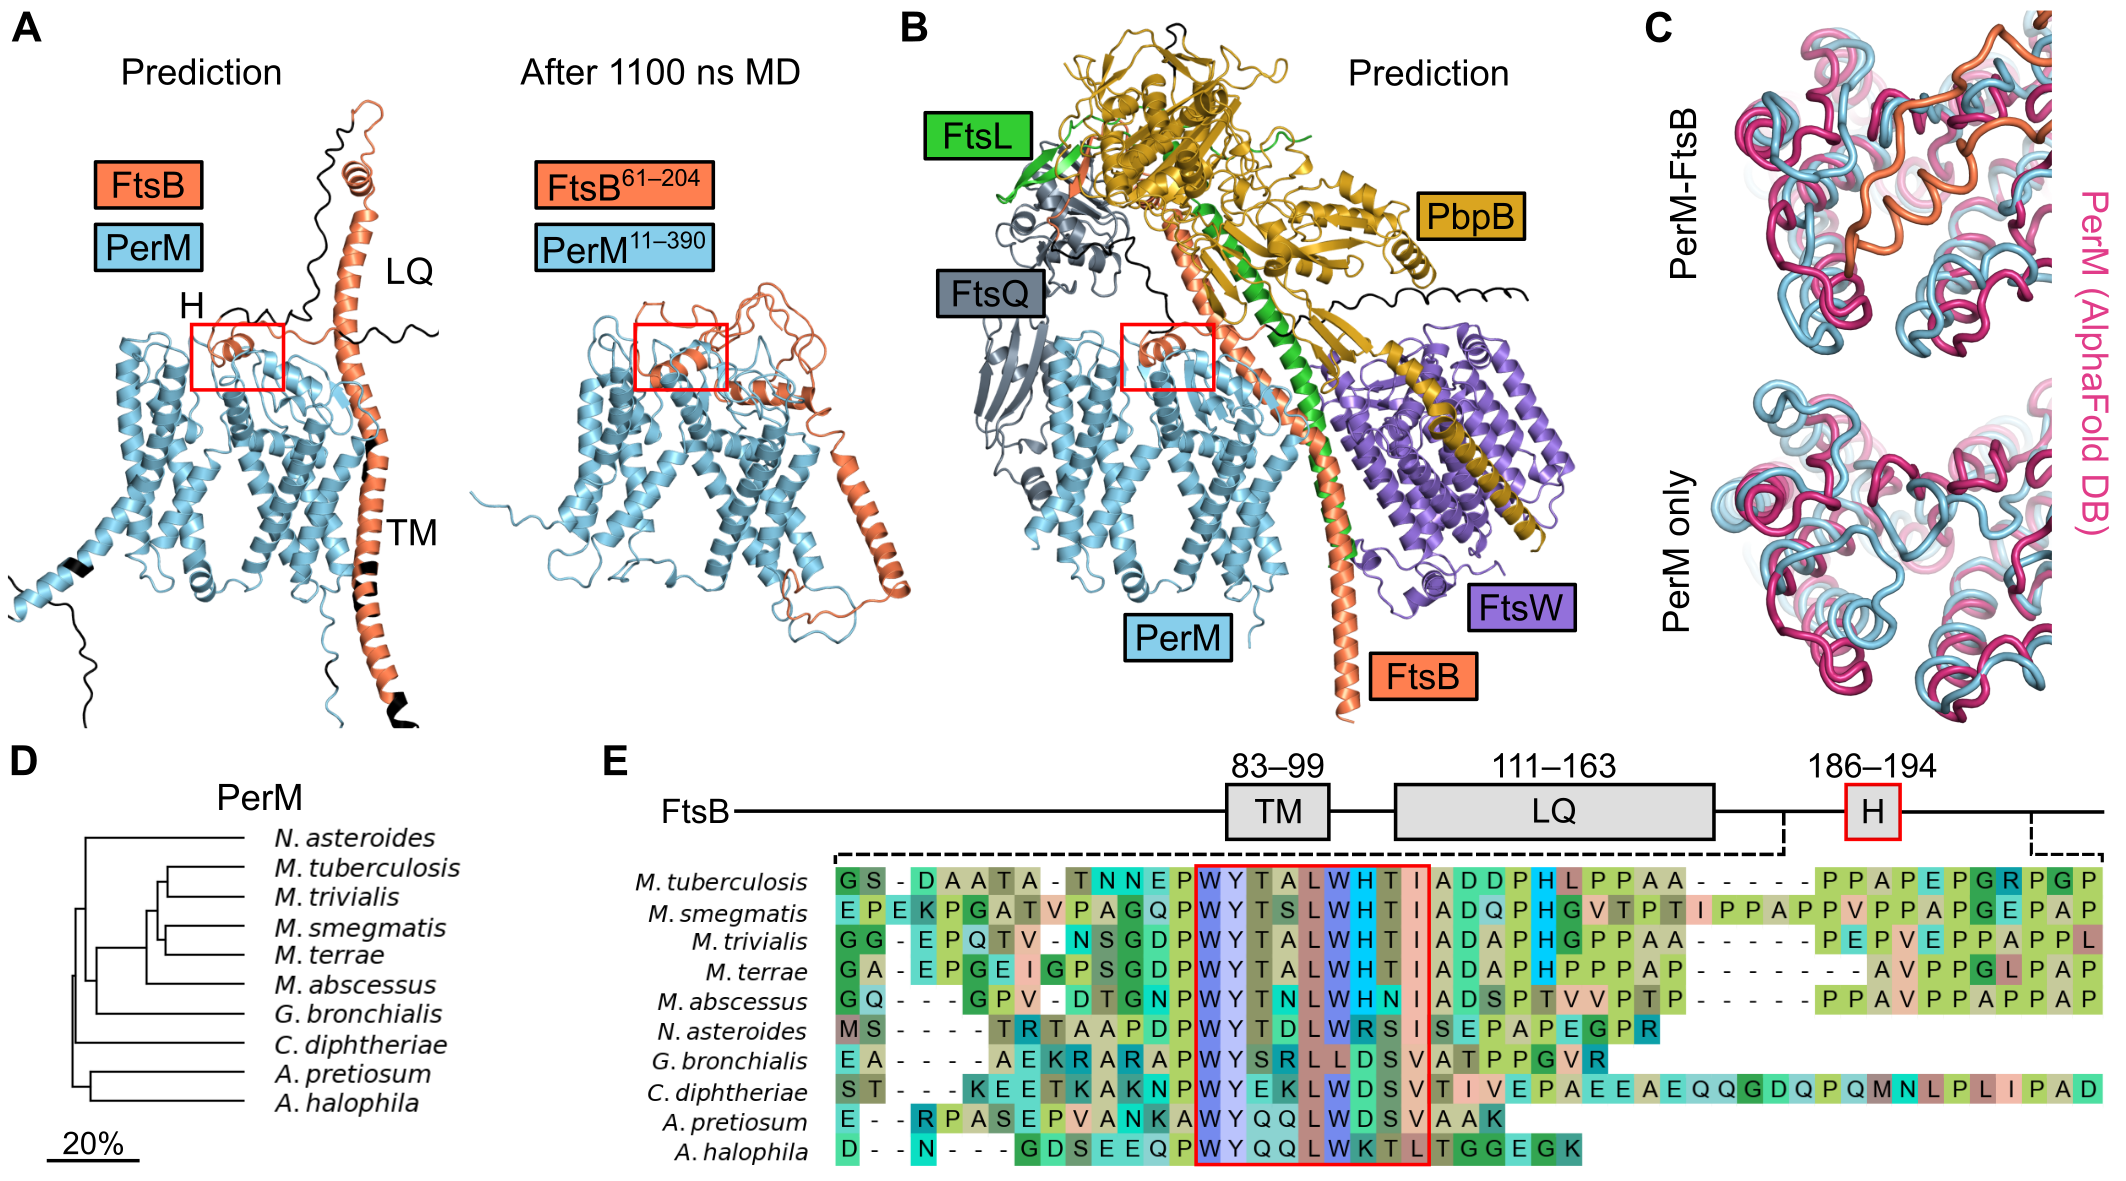
\includegraphics[width=1.0\textwidth]{../figures/fig1_1.png}
\caption{
    \textbf{A conserved, predicted \mtb{} PerM-FtsB interaction stabilizes PerM in MD.}
    (\textbf{A})~Left: predicted PerM-FtsB complex in which an $\alpha$~helix, \ftsbH{}, interacts with the periplasmic face of PerM. Transmembrane helix \ftsbTM{} and the region interacting with FtsL and FtsQ, \ftsbLQ{}, are indicated. Residues with $pLDDT < 50$ colored black. Right: final conformer following \qty{1.1}{\us} MD; PerM-\ftsbH{} interact persists, \ftsbLQ{} collapses, and \ftsbTM{} moves away from PerM.
    (\textbf{B})~Prediction for the \mtb{} divisome with inclusion of PerM. Terminal regions with $pLDDT < 50$ are omitted except for the FtsB C-terminus. All complexes in \textbf{A} and \textbf{B} are aligned by PerM C$\alpha$ atoms; the red box is placed at the same position relative to PerM for comparison of \ftsbH{} movement.
    (\textbf{C})~Final MD conformers for PerM-FtsB and for PerM alone are aligned by PerM C$\alpha$ atoms and compared to a PerM prediction  (AlphaFold DB P9WKN3-F1-model{\_}v4).
    (\textbf{D})~Phylogenetic tree for actinomycete species with predicted PerM-FtsB interactions. Branch length scaled by divergence in amino acid identity in pairwise sequence alignments of PerM.
    (\textbf{E})~Top: Diagram of \mtb{} FtsB defining the \ftsbTM{}, \ftsbLQ{}, and \ftsbH{} regions. Bottom: Multiple sequence alignment of a region near the C-terminus of FtsB for actinomycete species illustrates conservation of residues in \ftsbH{} and diversity in FtsB C-termini.
}\label{fig1_1}
\end{figure*}

We also found that a prediction of the core \mtb{} divisome with the addition of PerM was consistent with PerM interacting with the core divisome without obviously disrupting interactions between core divisome components (Fig. \ref{fig1_1}B).
PerM was only predicted to interact with FtsB within this complex. Based on these predictions, we identified three regions of interest in \mtb{} FtsB: the predicted transmembrane helix, \ftsbTM{} (FtsB 83--99), the region predicted to interact with FtsL and FtsQ, \ftsbLQ{} (FtsB 111--163), and a span of hydrophobic residues forming an $\alpha$~helix predicted to interact with PerM, \ftsbH{} (FtsB 186--194).
Although C-terminal residues following \ftsbH{} were predicted to thread between the PbpB anchor and head domains, there were no high-confidence predictions for this region.

In order to see the impact of FtsB on PerM, we replicated the three-stage MD protocol using PerM alone.
Final conformers for PerM-FtsB and PerM simulations are shown in Fig.~\ref{fig1_1}C and compared to a recent PerM structure prediction from the AlphaFold Protein Structure Database \citep{varadiAlphaFoldProteinStructure2022}.
Surprisingly, we found that the final conformer of the monomeric PerM simulation differed more from the predicted PerM structure ($RMSD=\qty{3.47}{\angstrom}$) to a greater extent than final conformers in PerM-FtsB simulation replicates (\qty{2.50}{\angstrom} and \qty{2.21}{\angstrom}).
The largest structural changes were seen in the predicted \ftsbH{} binding pocket.

Since our structure prediction was informed by information encoded in multiple sequence alignments, we searched for and identified PerM orthologs in actinomycetes (Fig.~\ref{fig1_1}D).
For each, we also identified the corresponding FtsB sequence and predicted the structures of PerM-FtsB complexes.
In every species tested there was a predicted interaction between PerM and \ftsbH{} (Supplementary Fig.~\ref{figS1}). Further, there is little difference in the lengths of regions linking \ftsbLQ{} and \ftsbH{}.
We constructed a multiple sequence alignments of FtsB to investigate the basis for conserved, predicted PerM-FtsB interaction and found that \ftsbH{} was highly conserved (Fig.~\ref{fig1_1}E) with near perfect conservation of hydrophobic residues predicted to interact with PerM (W\textsuperscript{186}, Y\textsuperscript{187}, L\textsuperscript{190}, and W\textsuperscript{191}).

Next, we investigated the structural basis for specific PerM-FtsB interaction. Fig.~\ref{fig1_2} illustrates the evolution of the FtsB binding pocket in PerM.
In both simulation replicates, we observed that a large, hydrophobic binding pocket narrowed, particularly around FtsB W\textsuperscript{186}. 
Residues in the W\textsuperscript{186} binding pocket include PerM G\textsuperscript{228}, which was perfectly conserved in PerM sequences in species that we analyzed.
Remarkably, specific hydrogen bonds between PerM and conserved FtsW residues emerged, none of which were present in structure predictions.
Fig.~\ref{fig1_1}B shows that evolution of the PerM-FtsB binding interface was reproducible.

\begin{figure*}[h]
    \centering
    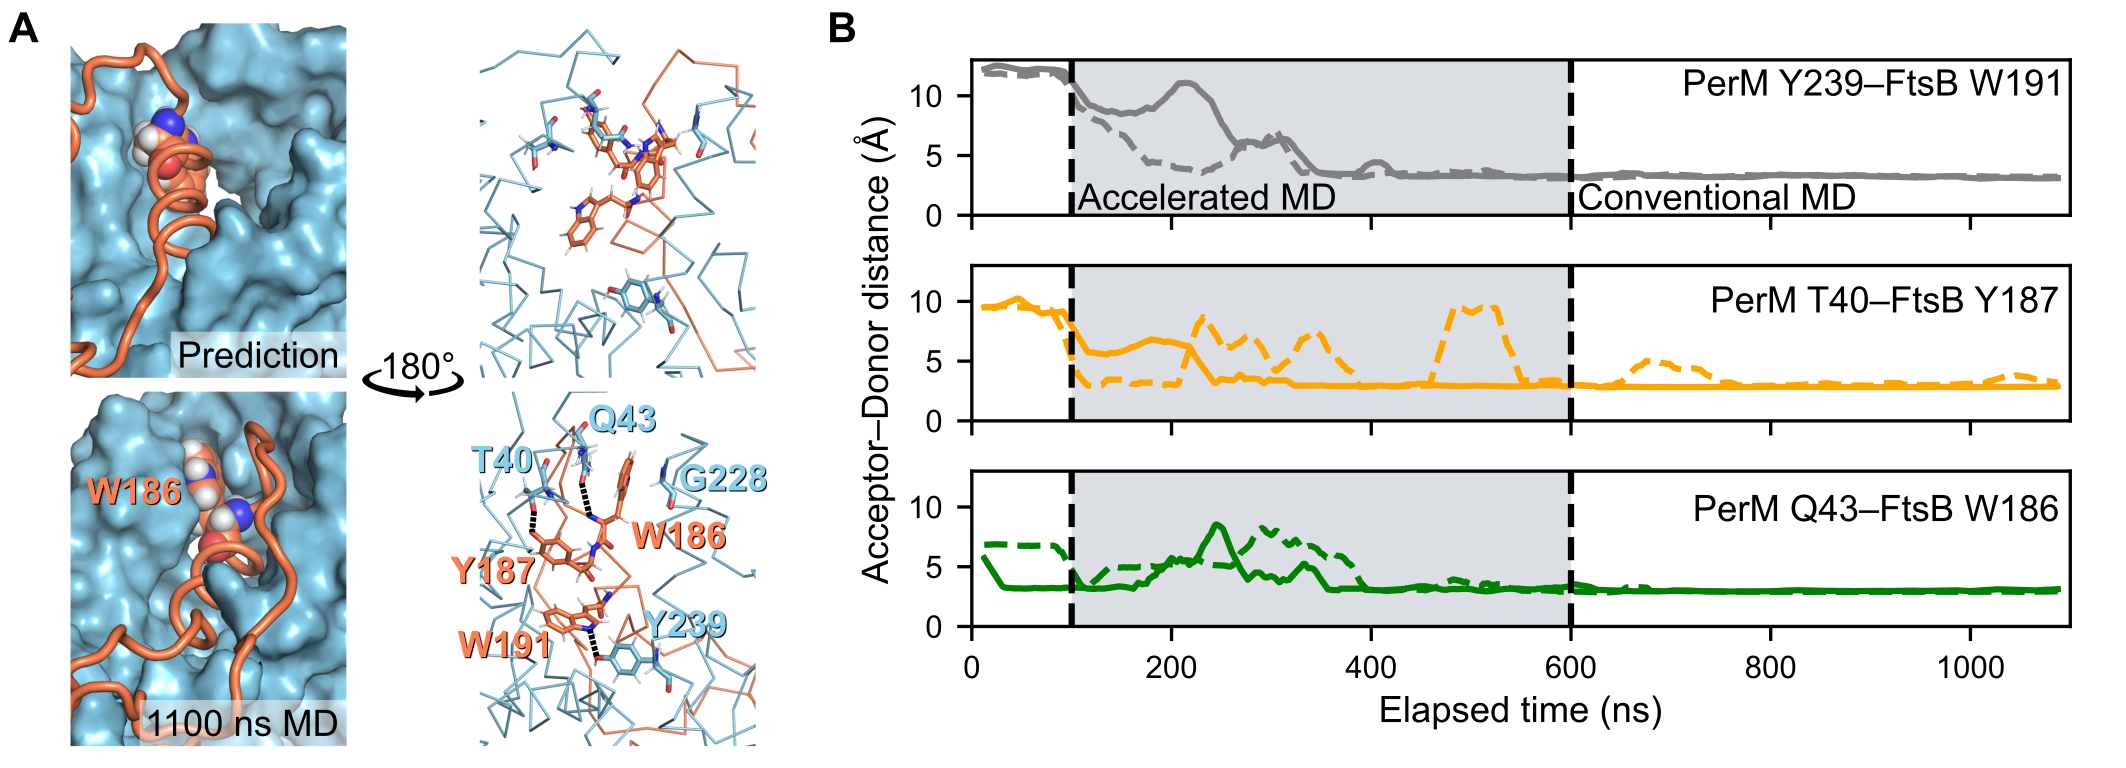
\includegraphics[width=1.0\textwidth]{../figures/fig1_2.png}
    \caption{
        \textbf{Reproducible dynamics at the PerM-FtsB binding interface.}
        (\textbf{A}) The shape of the FtsB binding pocket for PerM is compared between the predicted interface structure (top) and the final conformer following \qty{1.1}{us} MD (bottom). Left: a large predicted periplasmic binding pocket in PerM (top left) evolves to tightly bind FtsB W186 (bottom left). Right: Following MD (bottom right), FtsB W186 interacts with conserved PerM residue G228 and hydrogen bonds are formed between PerM and conserved FtsB residues. The same region is shown rotated by \qty{180}{\degree}.
        (\textbf{B}) Maturation of PerM-FtsB interactions were reproducible in MD. Solid and dashed lines show acceptor-donor distance (25-ns moving average; two MD replicates) for hydrogen bonds at the PerM-FtsB interface that are absent in the predicted structure.
    }\label{fig1_2}
\end{figure*}

\subsection{Transgenic expression of fluorescent FtsB and PerM constructs in \ec{}}

Despite the apparent specificity and stability of the predicted PerM-FtsB interface in MD, we wanted to confirm that this interaction does not depend on other \mtb{} components to be stable on timescales inaccessible by MD and, if so, to investigate whether \ftsbH{} mediated the interaction.
We constructed variants of FtsB with an N-terminal fusion of mTurquoise2 (mTq2-FtsB, mTq2-\ftsbdLQ{}, and mTq2-\ftsbdLQdH{}; Fig.~\ref{fig2}A). Deletion of \ftsbLQ{} clearly increased the FtsB expression level, suggesting instability of \mtb{} FtsB in the absence of FtsL and FtsQ.
However, FtsB instability in \mtb{} may result from other mechanisms \citep{wangPersistentMycobacteriumTuberculosis2019}, so we did not investigate this further.
We did not observe any further effect of deleting \ftsbH{}.

\begin{figure}[h]
    \centering
    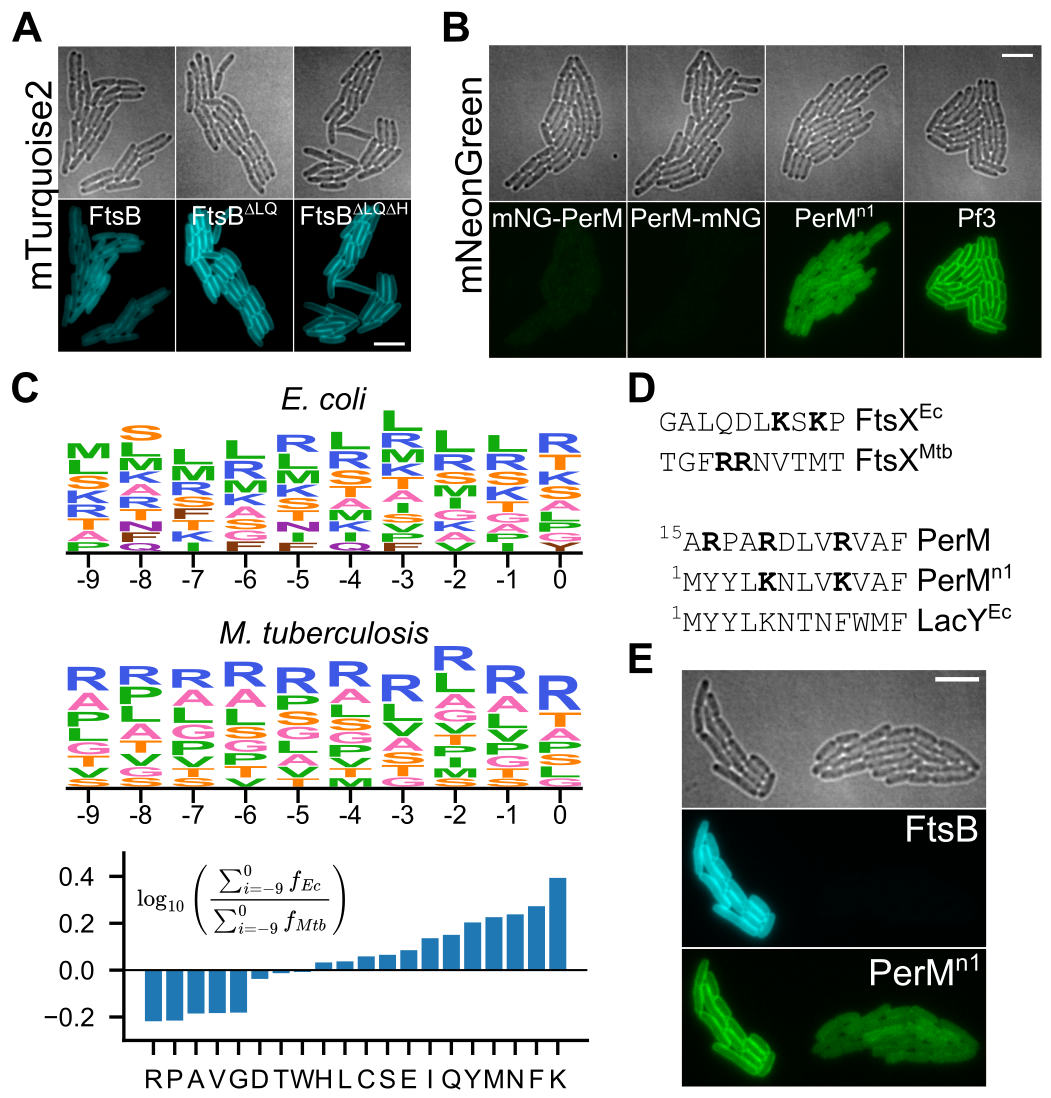
\includegraphics[width=0.5\textwidth]{../figures/fig2.png}
    \caption{
        \textbf{Expression of \mtb{} FtsB and PerM in \ec{}.}
        (\textbf{A}) Expression and membrane localization of FtsB and variants with deletions of \ftsbLQ{} or with deletion of both \ftsbLQ{} and \ftsbH{}. Identical minimum and maximum intensities for mTurquoise2 images.
        (\textbf{B}) Expression and membrane localization for mNG-PerM, PerM-mNG, \permN{}-mNG, and Pf3-mNG. Identical minimum and maximum intensities for mNeonGreen images.
        (\textbf{C}) Top: residue frequency for positions preceding the first predicted transmembrane helix, inclusive of residues found at frequencies above \qty{5}{\percent}. Letter height is proportional to residue frequency with more frequent residues on top. Bottom: relative frequencies in \ec{} and \mtb{}.
        (\textbf{D}) Top: residues preceding the first transmembrane helix in paralogs of FtsX, highlighting lysine and arginine residues. Bottom: comparison of PerM to \permN{} and \ec{} LacY.
        (\textbf{E}) Two adjacent microcolonies from a strain with co-expression of mTq2-FtsB and \permN{}-mNG. The microcolony on the right has coincidentally lost the plasmid encoding mTq2-FtsB, and exhibits reduced membrane localization of \permN{}-mNG. Scale bars \qty{5}{\um}.
    }\label{fig2}
\end{figure}

Conversely, initial attempts to construct mNeonGreen-labeled PerM failed for both N- and C-terminal fusion constructs (mNG-PerM and PerM-mNG; Fig.~\ref{fig2}B).
We manually inspected the predicted PerM structure as well as sequences of integral transmembrane protein orthologs in \ec{} and \mtb{}, hypothesizing that an engineered construct, \permN{}, would exhibit higher expression.
Specifically, we noticed an apparent ``LK'' motif in \ec{} that rarely appeared in \mtb{} and was reminiscent of part of the twin-arginine translocation motif \citep{leeBacterialTwinArginineTranslocation2006}.
Our strategy in designing the \permN{} construct was to modify PerM with aspects of the short LacY N-terminal sequence in ways that would not perturb the predicted PerM structure.
While expression was indeed much higher for \permN{}-mNG, it failed to exhibit the same degree of membrane localization as Pf3-mNG, which we used as a control given its efficient translocation and uniform transmembrane orientation \citep{kieferNegativelyChargedAmino1997}.

We were surprised at how much the modifications in \permN{} increased expression levels and systematically investigated sequences in residues preceding the first predicted transmembrane helix in all proteins including at least one transmembrane helix in \ec{} and \mtb{} (Fig.~\ref{fig2}C).
We found large differences in the frequencies of some residues, most strikingly for differences in the relative frequencies of lysine and arginine. Fig.~\ref{fig2}D shows how this is reflected in orthologous sequences of FtsX as well as in \permN{} compared to \mtb{} PerM.
Finally, we proceeded to co-express \permN{}-mNG and mTq2-FtsB and look for evidence of PerM-FtsB interaction.
Serendipitously, one of two adjacent \ec{} microcolonies in a co-expression experiment lost the plasmid for mTq2-FtsB expression (this occasionally happened without including selective antibiotics in agarose gel pads).
The large difference in \permN{}-mNG membrane localization between these two microcolonies suggested an unexpected role for FtsB in stabilizing PerM in the \ec{} membrane.

\subsection{PerM stabilization in \ec{} membrane by FtsB depends on \ftsbH{}}

In order to confirm that FtsB increases membrane-localized PerM expression and, if so, to investigate the role of \ftsbH{} in this phenomenon, we co-expressed mNeonGreen- and mTurquoise2-labeled constructs and analyzed fluorescence in \ec{} microcolonies (Fig.~\ref{fig3}). In these experiments, expression of \permN{}-mNG was induced with \qty{100}{\uM} IPTG. Localization controls mNeonGreen (strong cytoplasmic localization) and Pf3-mNG (strong membrane localization) were induced with \qty{60}{\uM} and \qty{240}{\uM} IPTG, respectively, to match typical \permN{}-mNG expression levels. Expression of mTurquoise2-labeled FtsB constructs was induced with \qty{10}{\nM} ATc in all conditions except for one condition with no induction (indicated with down arrows in Fig.~\ref{fig3}). Brightfield images of \ec{} cells were segmented, and protein concentration was estimated to be proportional to total integrated fluorescence after subtracting background and normalizing by cell size.

\begin{figure*}[h]
\centering
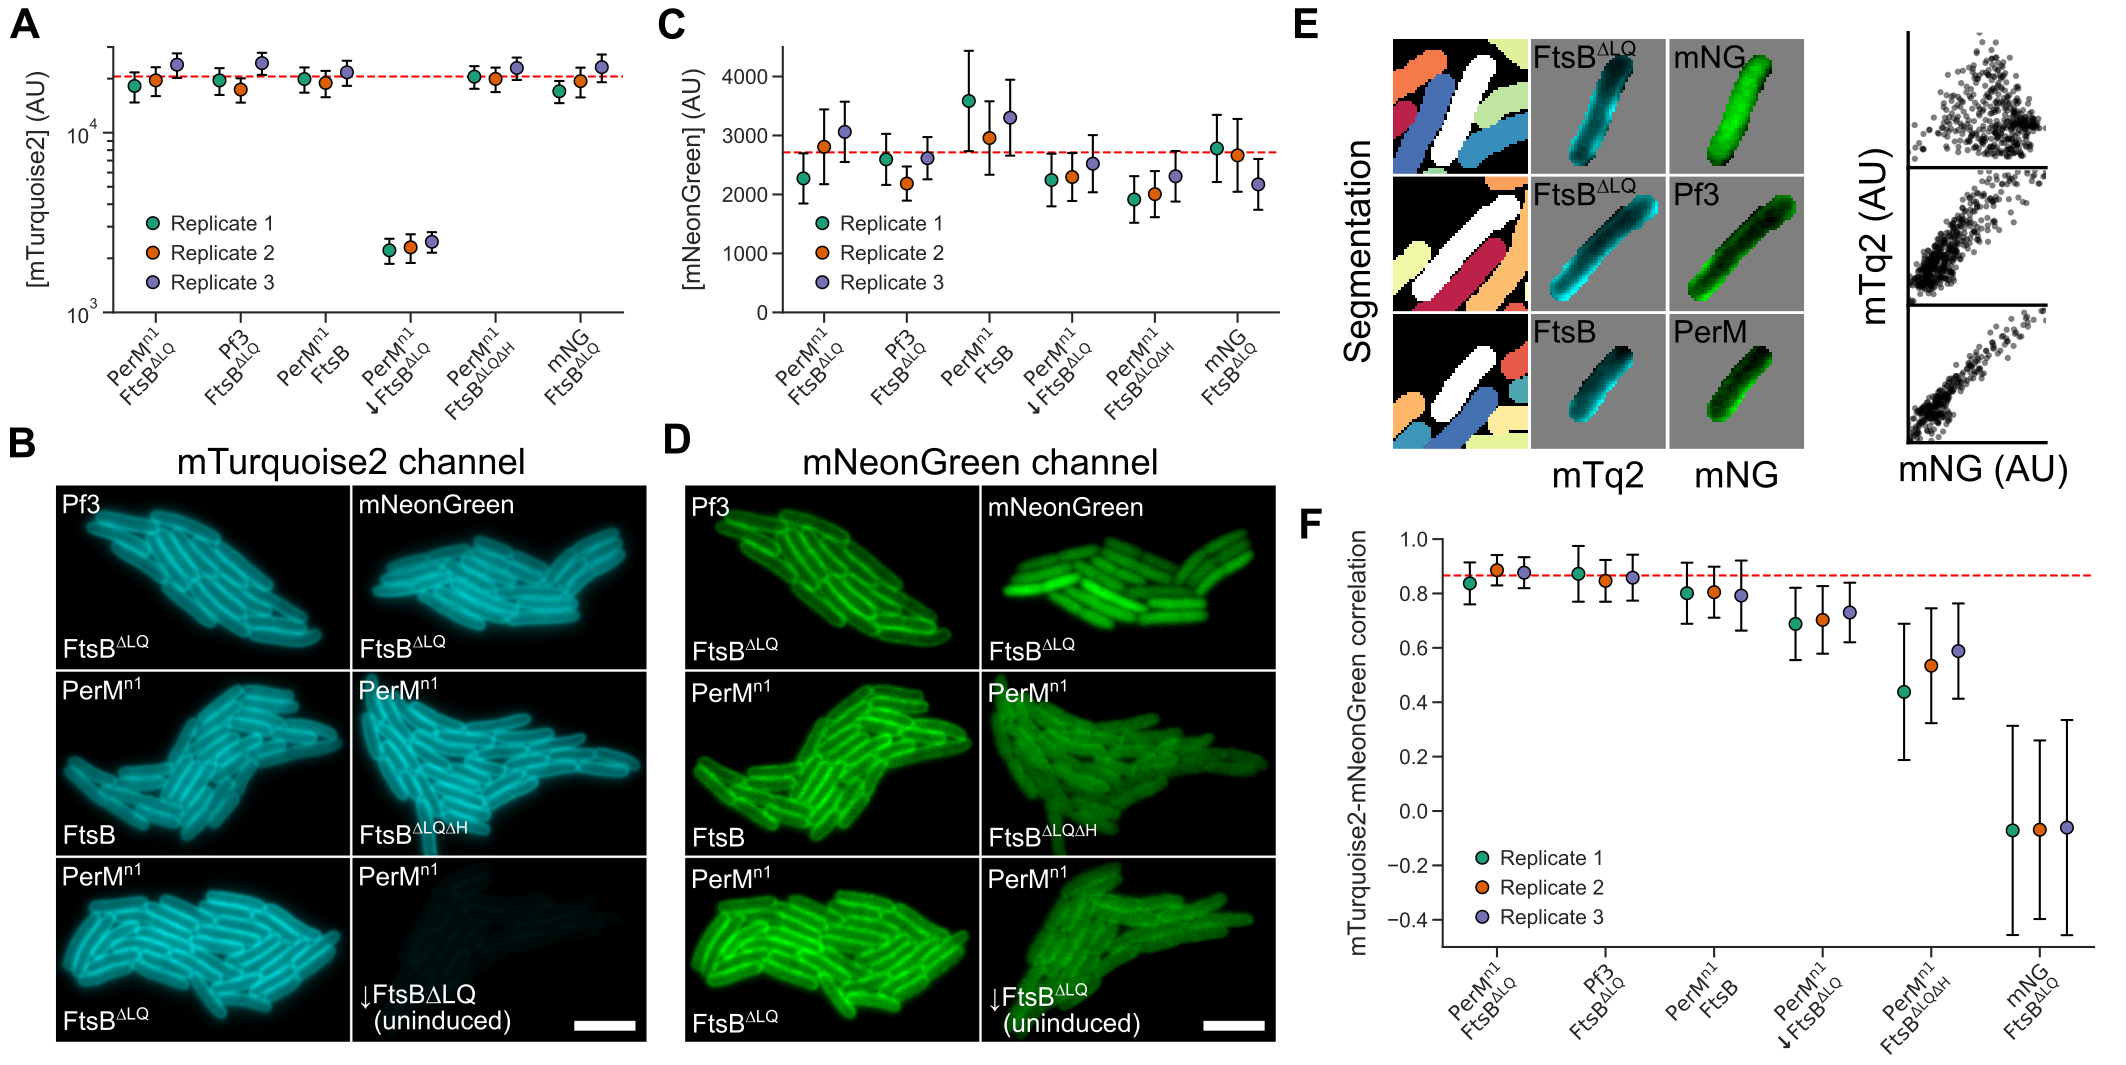
\includegraphics[width=1.0\textwidth]{../figures/fig3.png}
\caption{
    \textbf{FtsB stabilizes PerM in the \ec{} membrane.}
    (\textbf{A}) Distribution of single-cell mTurquoise2 concentration (mean $\pm$ standard deviation) for FtsB constructs in different conditions, each with replicates. Dashed red line indicates the mean value for the reference condition (\permN{}-mNG, mTq2-\ftsbdLQ{}, \qty{100}{\uM} IPTG, \qty{10}{\nM} ATc). Uninduced \ftsbdLQ{} is indicated with a down arrow. A logarithmic scale is used to allow comparison of high- and low-expression conditions.
    (\textbf{B}) Example data from microcolonies for each condition. The uninduced \ftsbdLQ{} condition has very low fluorescence in example data because identical minimum and maximum intensities were used. Scale bar \qty{5}{\um}.
    (\textbf{C, D}) Distribution of single-cell mNeonGreen concentrations and example data for Pf3-mNG, mNeonGreen alone, or \permN{}-mNG in different conditions; prepared identically to \textbf{A} and \textbf{B}.
    (\textbf{E}) Left: example data analysis showing cell segmentation and isolated, single-cell intensities. Right: Scatter plots of single-pixel intensities for each cell show clear correlation for Pf3-mNG and PerM-mNG, but not for mNeonGreen alone. (\textbf{F}) Distribution of single-cell Spearman correlation coefficients (mean $\pm$ standard deviation) for three replicates.
}\label{fig3}
\end{figure*}

Relative to the reference condition (\permN{} and \ftsbdLQ{}, \qty{10}{\nM} ATc), there was an \qty{89}{\percent} ($p=\num{3.3e-12}$) decrease in mTq2-\ftsbdLQ{} expression in the absence of induction, with no significant differences observed for other conditions. The absence of any significant impact on wild-type FtsB expression ($p=0.97$) compared to when FtsB was expressed in the absence of PerM (compare Fig.~\ref{fig3}B to Fig.~\ref{fig2}A) suggests that \permN{} stabilizes FtsB when expressed in \ec{}, as was observed in \mtb{} \citep{wangPersistentMycobacteriumTuberculosis2019}. There was also no obvious difference in localization of any FtsB variant in any condition tested.

In contrast, there was a significant reduction in \permN{}-mNG expression of \qty{13.3}{\percent} ($p=\num{3.8e-2}$) in the absence of induction of mTq2-\ftsbdLQ{} expression, and a reduction of \qty{23.5}{\percent} ($p=\num{5.5e-4}$) when \ftsbdLQ{} was replaced with \ftsbdLQdH{}. There was no significant change when \ftsbdLQ{} was replaced with wild-type FtsB ($p=0.29$). This suggested that FtsB increases PerM stability in \ec{}, and that this depends on the presence of \ftsbH{}. However, inspection of Fig.~\ref{fig3}C suggests that our sample size is overpowered ($N=\num{10930}$ cells in total from 3 replicates; $607 \pm 44$ cells per condition per replicate) given variation between replicates in mNeonGreen expression levels. 

In preliminary experiments, we observed a large decrease in spatial correlation between mTurquoise2 and mNeonGreen fluorescence when \ftsbdLQ{} was depleted or replaced by \ftsbdLQdH{} (Fig.~\ref{fig3}D). The observation of small reductions in mNG-\permN{} levels despite apparently large impacts of different FtsB constructs on localization suggested that fluorescent mNeonGreen often remained in the cytoplasm following mNG-\permN{} degradation. We hypothesized that quantifying spatial correlation would be a more sensitive measurement less susceptible to variation in protein expression levels. Fig.~\ref{fig3}E shows scatter plots of mNeonGreen and mTurquoise2 intensities for pixels in typical cells with cytoplasmic mNeonGreen, membrane-localized Pf3-mNG, and \permN{}-mNG. We calculated Spearman correlation coefficients from such distributions for segmented cells and Fig.~\ref{fig3}F shows the mean and standard deviation of correlation coefficients for each condition and replicate.

In the reference condition (\permN{}-mNG, mTq2-\ftsbdLQ, \qty{10}{nM} ATc), correlation was high ($\rho = 0.87$, 0.84--0.89 \qty{95}{\percent} confidence interval) and indistinguishable from that when Pf3-mNG was expressed instead ($p = 0.72$). All other conditions had significant reductions in correlation. Wild-type FtsB was marginally less well correlated ($\rho = 0.80$, 0.77--0.83). The apparent reductions in \permN{}-mNG expression levels discussed above were more strongly supported by analysis of spatial correlation, with a drop in correlation in the absence of mTq2-\ftsbdLQ{} induction ($\rho = 0.71$, 0.69--0.73) and a larger drop when mTq2-\ftsbdLQ was replaced with mTq2-\ftsbdLQdH ($\rho = 0.52$, 0.46--0.58). While \ftsbLQ{} was not absolutely essential for membrane localization of \permN{}, this was also observed in the absence of any FtsB expression (Fig.~\ref{fig2}B).

\subsection{Single-molecule FtsB tracking}

Our correlation analysis strongly suggested that FtsB interaction with PerM via \ftsbH{} is key for expression of \permN{} in the membrane. Since we observed this for transgenic expression in \ec{}, it is unlikely that PerM-FtsB interaction is mediated by host proteins. However, transient PerM-FtsB interaction could be sufficient for PerM stability without a large fraction of molecules being bound at any time. If PerM is a significant component in the core \mtb{} divisome as suggested by depletion phenotypes and midcell localization \citep{goodsmithDisruptionTuberculosisMembrane2015, wangPersistentMycobacteriumTuberculosis2019}, we hypothesized that this implied long-lived PerM-FtsB interactions that could be detected by single-molecule tracking of FtsB diffusion. FtsB has a single transmembrane helix and PerM is predicted to have 8 (Fig.~\ref{fig1_1}A), suggesting an expected reduction in the FtsB diffusion coefficient from approximately 0.7 to \qty{0.3}{\square\um\per\s} upon PerM binding \citep{lucenaMicrodomainFormationGeneral2018}.

Describe methods concisely in way that makes sense. Why SASPT?
Robust against variable trajectory length and defocalization effects.
Describe very clearly limitations of apparent diffusion coefficient.

\loremipsum{}

Check out Fig. \ref{fig4}!

\begin{figure*}[h]
\centering
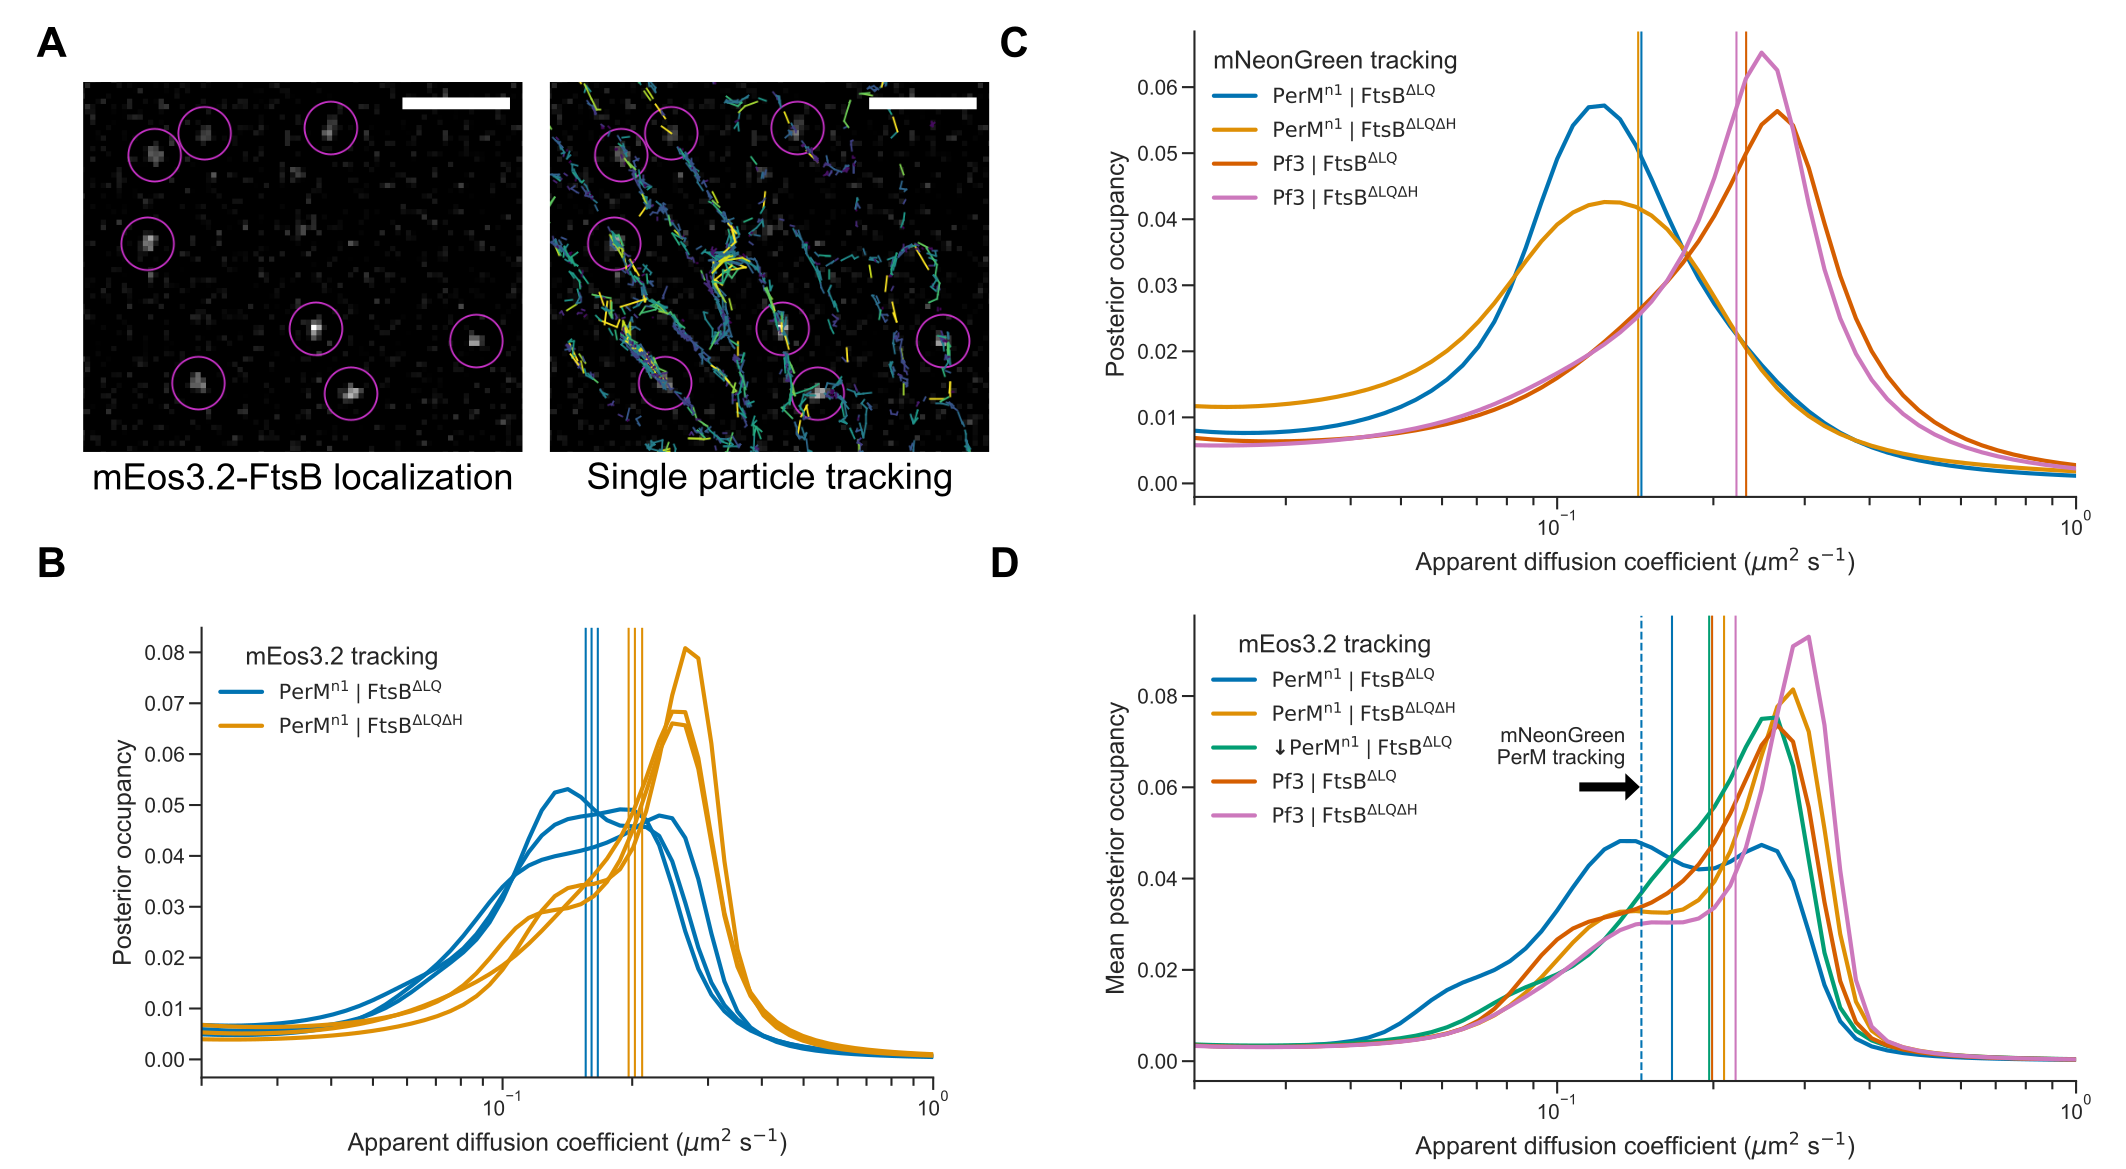
\includegraphics[width=1.0\textwidth]{../figures/fig4.png}
\caption{
    \textbf{PerM-FtsB binding detected by FtsB single-molecule tracking.}
    (\textbf{A}) Left: single, 33-ms frame from a fluorescence microscopy movie of mEos3.2-\ftsbdLQ{} diffusion in \ec{}. Right: Single-molecule localization and tracking results for the entire movie show membrane-localized diffusion. Scale bar $2~\mu$m.
    (\textbf{B}) Posterior occupancies in a model of regular Brownian motion and localization error were marginalized over localization error to estimate the distribution of apparent 2D diffusion coefficients. Distributions and their means (dashed lines) are shown for three replicates of experiments combining \permN{}-mNG with either mEos3.2-\ftsbdLQ{} or mEos3.2-\ftsbdLQdH{}.
    (\textbf{C}) Estimated distributions of diffusion coefficients inferred from single-molecule tracking of either \permN{}-mNG or Pf3-mNG with either \ftsbdLQ{} or \ftsbdLQdH{} (single experiment). Vertical lines indicate the mean estimated diffusion coefficient for each condition.
    (\textbf{D}) Estimated distribution of diffusion coefficients for either mEos3.2-\ftsbdLQ{} or mEos3.2-\ftsbdLQdH{} co-expressed with either Pf3-mNG or \permN{}-mNG (with or without addition of 100~$\mu$M~IPTG), inferred from combining data from three replicates. Vertical lines indicate mean estimated diffusion coefficients and the dashed vertical line is replicated from \textbf{C}.
}\label{fig4}
\end{figure*}

\subsection{Complex MD (fig 5)}

Tilt angles.
19.2 degrees from AF2 prediction compared to 21 degrees observed for Pa cryo-EM structure and ~20 degrees for various E. coli divisome molecular dynamics simulations.
4.8 degrees is reversion towards the AF2 prediction with the loss of PerM-FtsB interaction.

\loremipsum{}

\begin{figure*}[h]
\centering
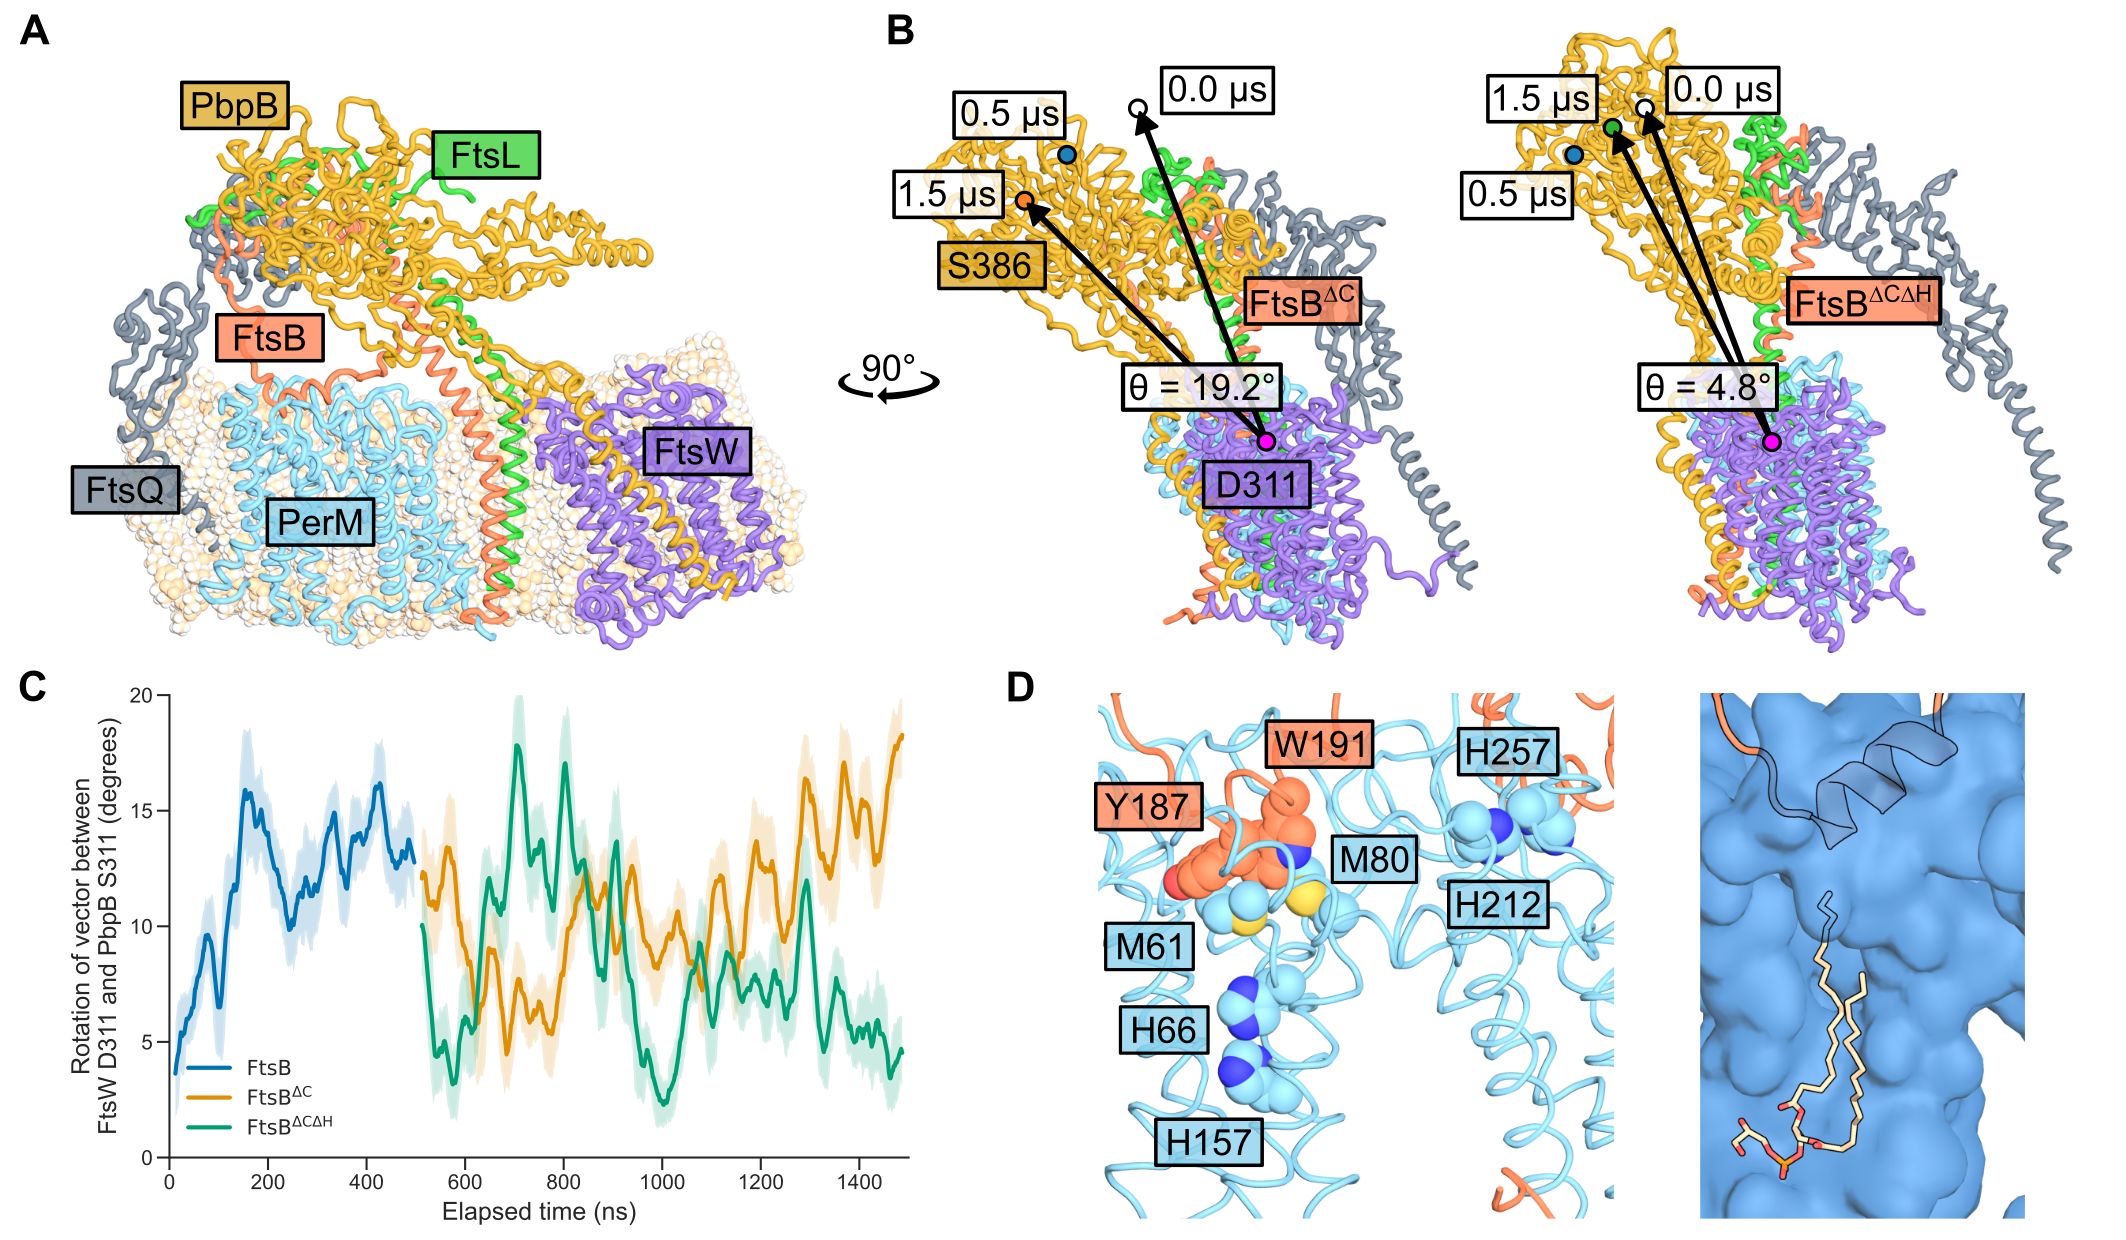
\includegraphics[width=1.0\textwidth]{../figures/fig5.png}
\caption{
    \textbf{PerM-FtsB interaction constrains the \mtb{} divisome in MD simulations.}
    (\textbf{A}) PerM simulated in context of \mtb{} divisome. Final conformer following \qty{1.5}{us} total MD. Note C-terminal truncation of FtsB relative to the predicted structure in \ref{fig1_1} that is uncertain in this region.
    (\textbf{B}) Difference in tilt of PbpB transpeptidase domain relative to its conformation in structure prediction.
    (\textbf{C}) Dynamics of tilt angle. (\textbf{D}) Left: residues in PerM near FtsB-binding interfaces suggest potential regulatory signals. Right: a lipid often fills a channel in PerM reaching FtsB.
}\label{fig5}
\end{figure*}

Note region initially predicted and used for MD.

Fig.~\ref{fig5}D shows the final conformer of the PerM-FtsB simulation to highlight interactions of interest.
A lipid tail occupies a channel in PerM and heavy-atom contacts with a POPG within \qty{5}{\angstrom}.

\section{Discussion}

Apparent diffusion coefficient. Future work will collect 3D data to investigate displacement along the surface of the membrane at any position.

\subsection{Mechanism discussion}
\citep{kashammerCryoEMStructureBacterial2023} discuss elongated conformation as potentially reflecting the catalytically active state.
Within the context of this model and in light of our results, the role of PerM would be to reduce divisome activity by constraining PbpB in a tilted conformation. 
An apparent paradox given that PerM is essential in some conditions in \mtb{} and in \msmegfull{}.
One hypothesis that can resolve this paradox is that PerM plays a conditionally essential role in promoting FtsB stability (which can be bypassed with FtsB overexpression \citep{wangPersistentMycobacteriumTuberculosis2019}) as well as a role in regulating divisome activity.
Residues that could potentially sensitize PerM-FtsB interaction are highlighted in Fig.~\ref{fig5}D.
Buried pair of histidines potentially play a role in tuning cell-division activity in response divalent cation concentrations, consistent with PerM first being described for its Mg\textsuperscript{2+}-dependent growth defect \citep{goodsmithDisruptionTuberculosisMembrane2015}.
Furthermore, in MD we routinely observed lipids to penetrate the first half of PerM and come into contact with FtsB, suggesting the possibility that bilayer composition can directly impact PerM-FtsB interaction.

Remaining questions. C-terminal residues. Note that C-terminus is not widely conserved. Prediction uncertain.

% Recap 

% Limitations

% Overall conclusion

\section{Methods}

\subsection{Structure prediction}

colabfold.
mmseqs2.
AF2-multimer.

Orthologous complexes.
mmseqs2 unpaired and paired sequences from reference sequences and environmental sequencing
alphafold2 multimer v3
12 recycles
model 4

Pymol for visualization.

\loremipsum{}

\subsection{Molecular dynamics}

PerM-FtsB simulations.
System details.
Simulation methods.
Analysis RMSD.
Analysis H bond distance.

Divisome simulation. System details. Simulation methods. Active site residue positions. Angle and PerM distance calculations.
Initial 500 ns simulation included full FtsB C-terminus

\loremipsum{}

\subsection{Sequence analysis}

Identification of diverse species with PerM-FtsB interactions by searching for PerM homologs.
Multiple sequence alignment.

\loremipsum{}

\subsection{Strains}

Cloning details.
Strain list.

\loremipsum{} 

\subsection{Microscopy}

Cell growth is same for both types of images.
Sample preparation.
Microscope details.

\loremipsum{}

\subsubsection{Microcolony fluorescence imaging}

Sample size.

\loremipsum{} 

\subsubsection{Single-molecule tracking}

\loremipsum{} 

\subsection{Image analysis}

ImageJ/Fiji reference for image preparation.

Test test test

\loremipsum{}

\subsubsection{Inference of diffusion coefficient distributions}

SASPT details.
Brief discussion of apparent 2D diffusion and challenge of identifying perfect method.
Details needed to define reported values.
Robustness checks with preliminary data: (1) MSD results similar to jump-distribution fitting similar to SASPT, (2) imaging near membrane/coverslip interface vs focused at midplane of cell gave apparent diffusion coefficients almost twice as high as expected.
Robustness checks for fitting: (1) Number of iterations for inference. (2) Fixing localization error to \qty{25}{nm}, (3) excluding trajectories longer than 10 frames that can be long-lived artifacts, (4) excluding trajectories with only 2 frames that can be mistakenly linking different molecules or false positive detections.
Normalizing inferred likelihoods of diffusion coefficients between 0.02 and 1.0 based on preliminary observations.
\qty{0.02}{\square\um\per\s}

\loremipsum{} 

\subsubsection{Microcolony fluorescence correlation}

Background estimation and substraction. Does not effect correlation by definition.
Segmentation of brightfield images with Omnipose.
Image registration. Important.

\loremipsum{} 

\subsection{Statistical analysis}

For mNeonGreen and mTurquoise2 concentration and correlation comparisons, a mixed linear model was fit to data points from single cells with random slopes and intercepts to allow for day-to-day variation. Two-tailed p-values were calculated for comparison to the reference condition (\permN{} and \ftsbdLQ{}, 100~nM~ATc) and adjusted for multiple comparisons using the Holm-Šidák method. Effect sizes are reported for significant results only (adjusted $p<0.05$). Unless stated otherwise, errors in the manuscript are 1 standard error of the mean.

\loremipsum{}

\backmatter

\bmhead{Acknowledgements}

FUNDING. HELP IN LAB (SMC). HELP IN WRITING AND REVIEW. ANY PLASMIDS/REAGENTS?

\bmhead{Resource availability}
Plasmids described in this manuscript will be made available through AddGene shortly.
Analysis code on GitHub.
Data available on request and will be archived to Zenodo following peer review.

\bmhead{Author contributions}

JF: molecular cloning, data acquisition, preliminary data analysis and interpretation. RX: data acquisition, data analysis. ZH: management, structure predictions and simulation, data acquisition, data analysis. All authors wrote and edited the manuscript.

\bibliography{perm-ftsb}% common bib file

\begin{appendices}

\section{Supplementary Figures and Tables}

\begin{figure*}[h]
\centering
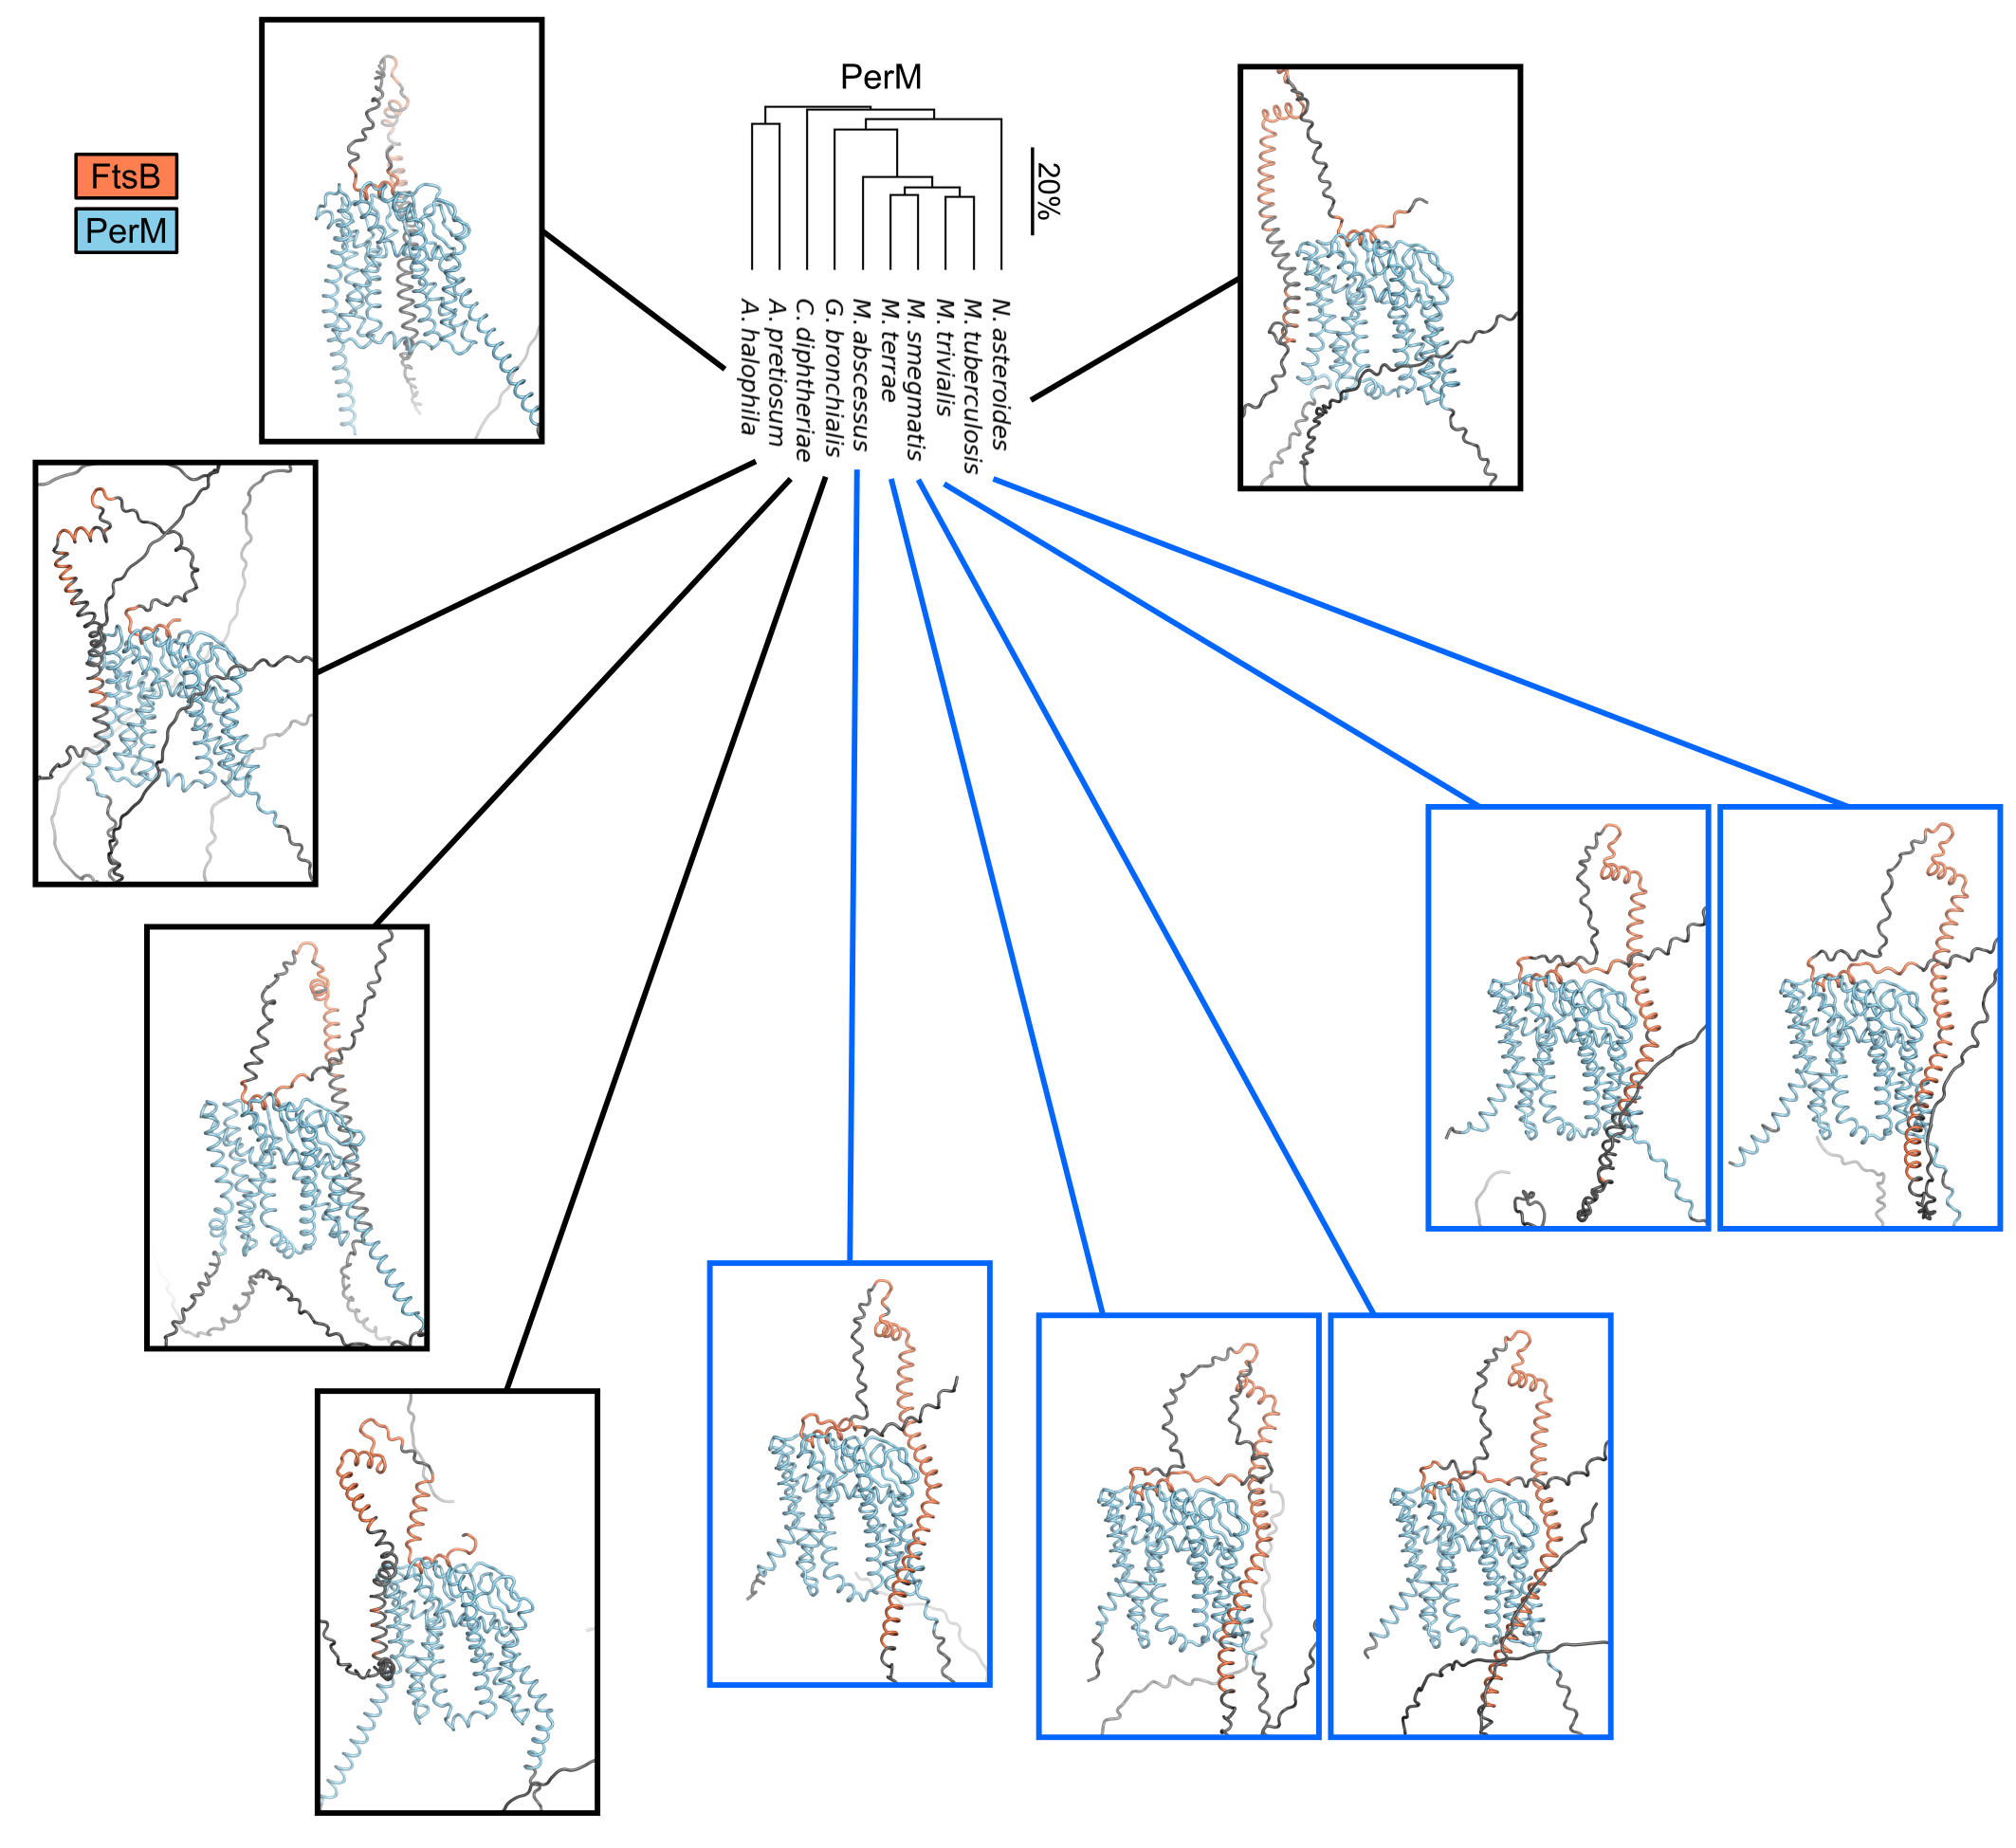
\includegraphics[width=1.0\textwidth]{../figures/figS1.png}
\caption{The PerM phylogenetic tree from Fig.~\ref{fig1_1} is reproduced and compared to PerM-FtsB complexes predicted from full-length sequences for the same species. The predicted orientation of \ftsbTM{} relative to PerM observed for \mtb{} is only observed for more closely related species (blue lines). However, \ftsbH{} interaction with PerM is predicted for all species. Residues with $pLDDT<50$ are colored gray.}\label{figS1}
\end{figure*}

\end{appendices}

\end{document}
